\chapter{Preliminaries}\label{ch:preliminaries}


\section{SpecElicitor}

SpecElicitor is a tool made by Yuan-Hong Lo, 
which can help user test Mobile Application with friendly GUI interface.

When user start using SpecElicitor,
each time user do an action on the Mobile Application, 
the tool will ask for labeling the action and the screen shown on the interface.
The interface is shown in Fig[].
By using SpecElicitor, we can choose the specified action at every step, label the meaning of the action,
and label the exception situation if it happen and stop the trace at any time we need.
The interface of the SpecElicitor is shown in Fig[\ref{SpecElicitorInterface}].


The traces made by SpecElicitor include automata, screenshots, XML files and labels.
The automata is a json file record every states and edges on the traces.
A state has a screenshot and a XML file dumped from the Mobile,
and an edge records the action user did such as clicking element, typing text or exiting the Application.
The traces also record labels on every states and edges,
so we can recognize how many label we focus on happened on the trace.
An example trace of Recipe Application made by SpecElicitor is shown in Fig[\ref{SpecElicitorTraces}].

%Our LAb 建立了一個工具SpecElicitor
%使用者可以在GUI介面下一邊建立APP的trace, 同時標記該畫面/動作的label
%使用完後會產生含有 XML, 截圖, label的traces

\begin{figure}[ht]
	\graphicspath{{pic/}}
	\begin{center}
		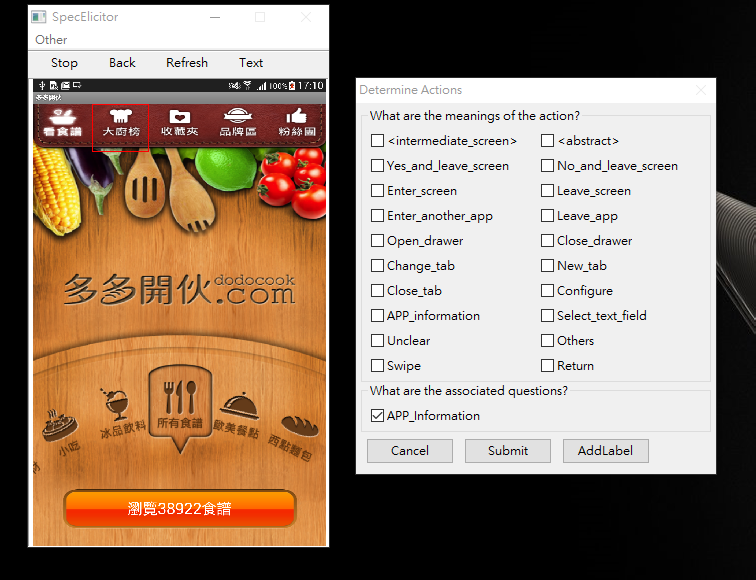
\includegraphics[width=0.8\textwidth]{SpecElicitorInterface.png}
		\caption{ The GUI interface of SpecElicitor.  }
		\label{SpecElicitorInterface}
	\end{center}
\end{figure}

\begin{figure}[ht]
	\graphicspath{{pic/}}
	\begin{center}
		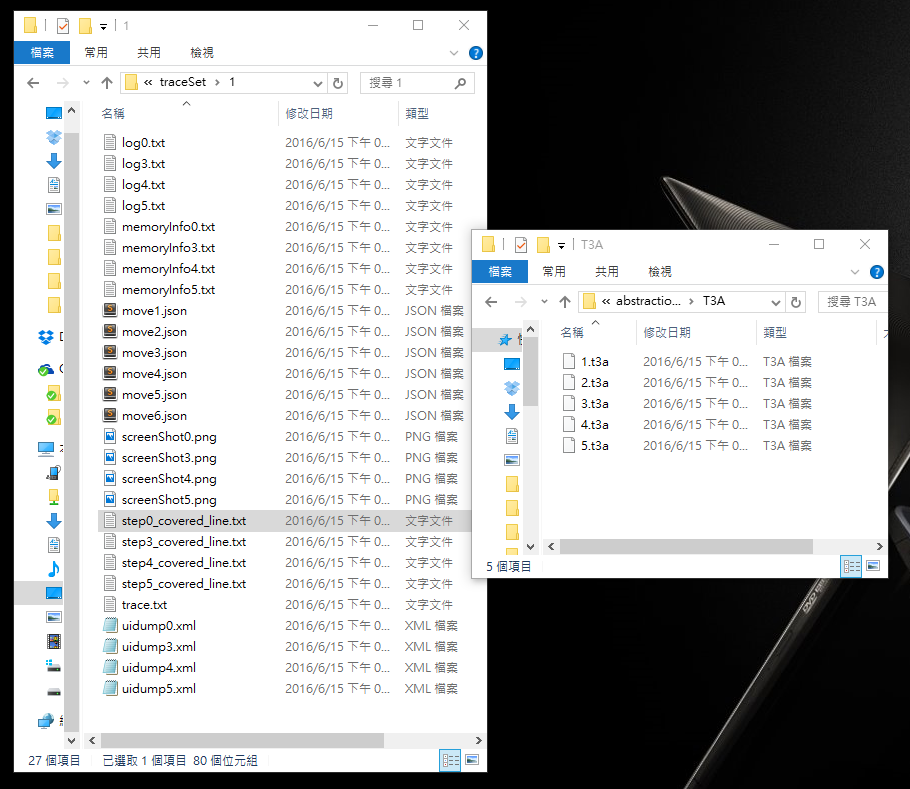
\includegraphics[width=0.8\textwidth]{SpecElicitorTraces.png}
		\caption{ An example of the traces.  }
		\label{SpecElicitorTraces}
	\end{center}
\end{figure}

\clearpage

\section{Common Sense Label}

將APP建立出state-base的automata,其中screen作為state,action作為edge

用統一的normalized terms來specific

our Lab建立一個TAAD的SpecElicitor,可產生label的trace


\section{Support Vector Machine}

SVM 在高維度 用largest margin來 seperate datas 

SVM可用來 cluster data